\index{general}{Free Surface}


When carrying out global models, typically  mantle convection, the effect of the free surface
is often neglected/negligeable: topography ranges from $\sim$ 10km depth to $\sim$ 10km height, which 
is very small compared to the depth of the mantle ($\sim$ 3000km). 

However, it has long been regognised that there is a feedback between topography and crust/lithosphere
deformation: the surface of the Earth reflects the deeper processes, from orogeny, back-arc basins, 
rifts, mid-ocean ridges, etc ... (see for instance \cite{brau10}).

\begin{remark}
Free surface flows are not unique to Earth sciences, and their modelling has given rise to many studies 
and textbooks. A typical free-surface flow problem in the CFD literature is the so-called 'dam break' 
problem \cite{moeb99,bacp07,liir07,lemx08,homa09,anco09}. Other occurrences involve 
sea waves, flow over structures, flow around ships, mould filling, flow with bubbles \cite{liir07}.
\end{remark}
 
What distinguishes geodynamics free surface modelling from its engineering 
counterpart is (i) the absence of surface tension, (ii) the fact that the fluids under consideration are
Stokesian, (iii) their rheology is complex (the elastic and plastic components can be 
dominant at the surface).

%There are to main modelling approaches employed in Computational Geodynamics: the so-called 
%'sticky air' approach and the Arbitrary-Lagrangian approach.

The problem of dealing with a free surface can be deceptively simple at first glance: as mentioned before the
amplitude of surface movement is often less than 1\% of the domain size. Isostacy-driven movements are
easy to deal with since the movement is vertical (and often characteried by  long wavelength). However, computational 
problems quickly arise in subduction modelling: the downgoing lithosphere subducts below the 
overriding plate and the relative convergence of the two is likely to generate a cusp at the trench. The presence
of shear bands intersecting the surface accentuates the problem:

\begin{center}
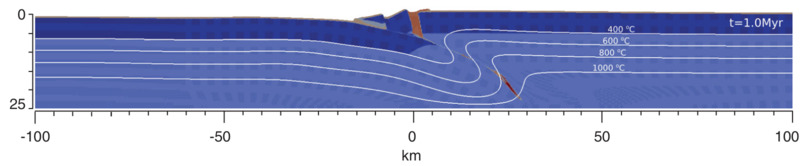
\includegraphics[width=13cm]{images/freesurface/matv15} \\
{\tiny Taken from Maffione et al \cite{matv15}. Example of free surface deformation above 
intra-oceanic subduction initiation}
\end{center}

\begin{remark} It is difficult to talk about free surface without including the underlying mesh. What follows
should be read alongside Section~\ref{sec:meshes}.
\end{remark}

%.......................................
\subsubsection{The fully Lagrangian approach}

\index{general}{Bow-tied element}

In this case the mesh is deformed with the velocity (or displacement) computed on its nodes. 
It is sometimes called 'body fitting' \cite{crsg12} or 'boundary fitted'. 
In the case when large deformation occurs (which is rather frequent in geodynamics - 
think about subduction or rifting processes where materials end up moving 100's or 1000's of km, horizontally
and/or vertically), it leads to highly deformed elements, and in some case even bow-tied:

\begin{center}
\frame{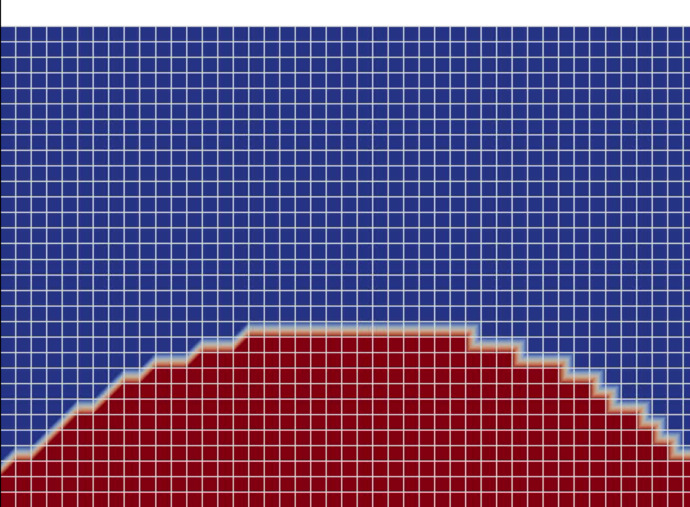
\includegraphics[width=4.5cm]{images/freesurface/b00}}
\frame{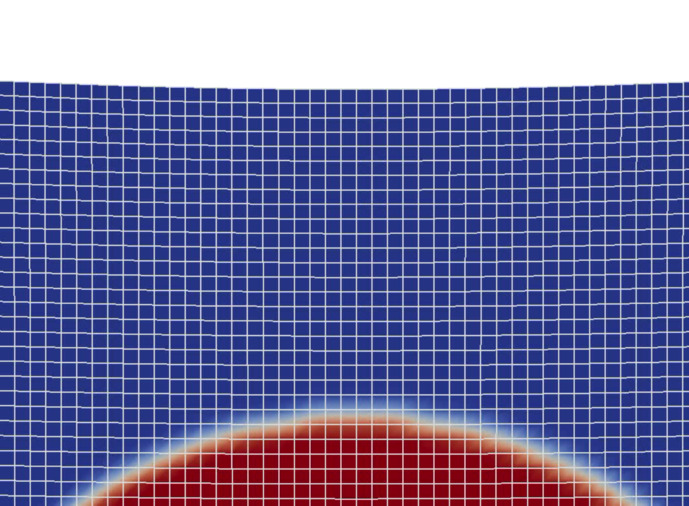
\includegraphics[width=4.5cm]{images/freesurface/b01}}
\frame{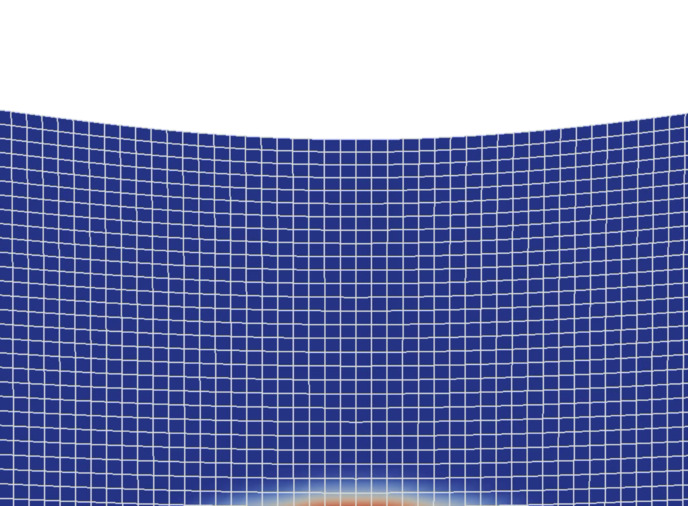
\includegraphics[width=4.5cm]{images/freesurface/b02}}\\
\frame{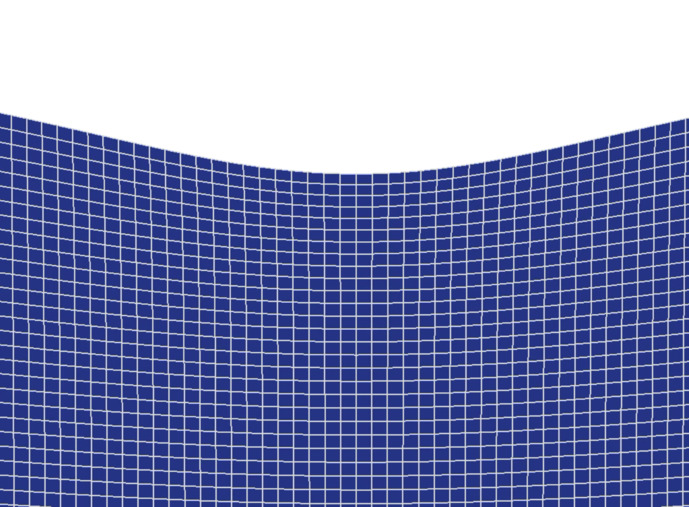
\includegraphics[width=4.5cm]{images/freesurface/b03}}
\frame{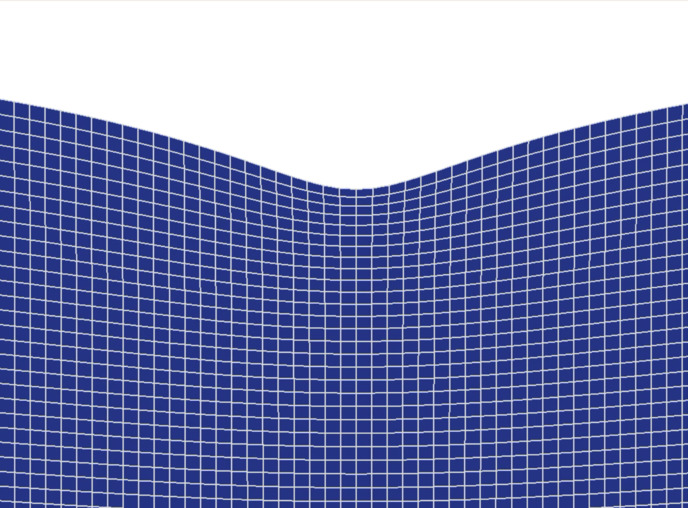
\includegraphics[width=4.5cm]{images/freesurface/b05}}
\frame{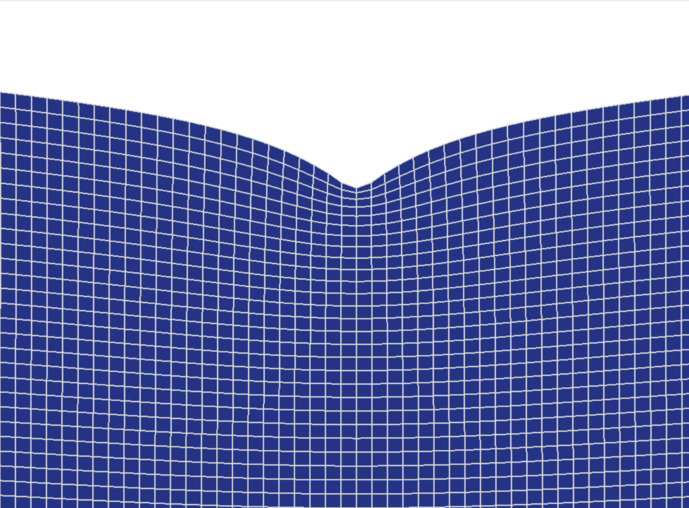
\includegraphics[width=4.5cm]{images/freesurface/b07}}\\
\frame{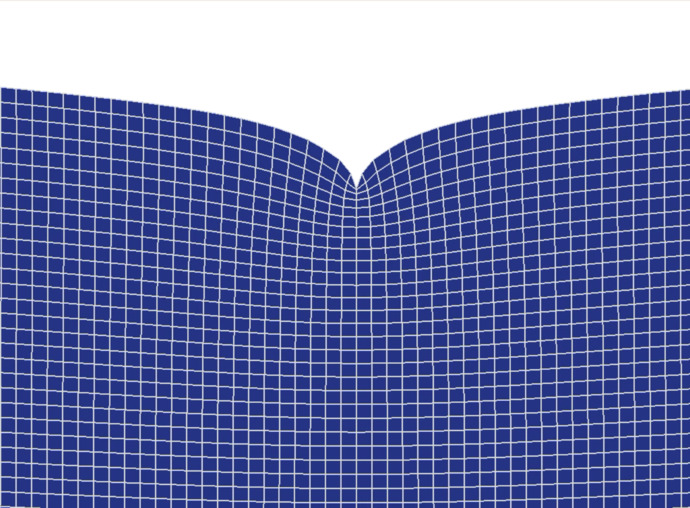
\includegraphics[width=4.5cm]{images/freesurface/b08}}
\frame{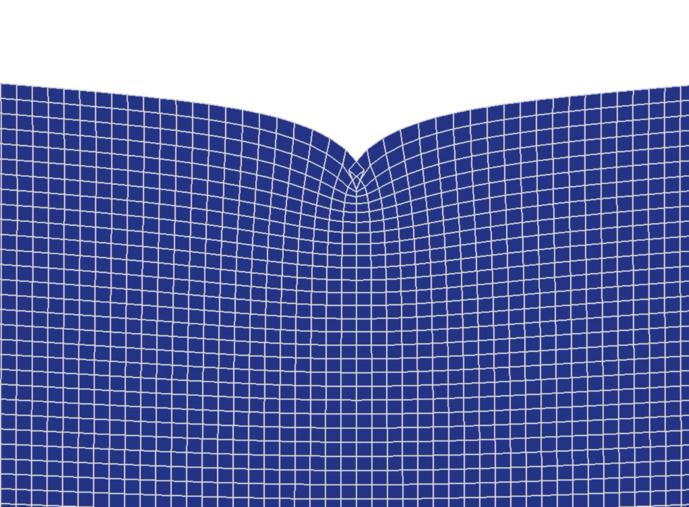
\includegraphics[width=4.5cm]{images/freesurface/b09}}
\frame{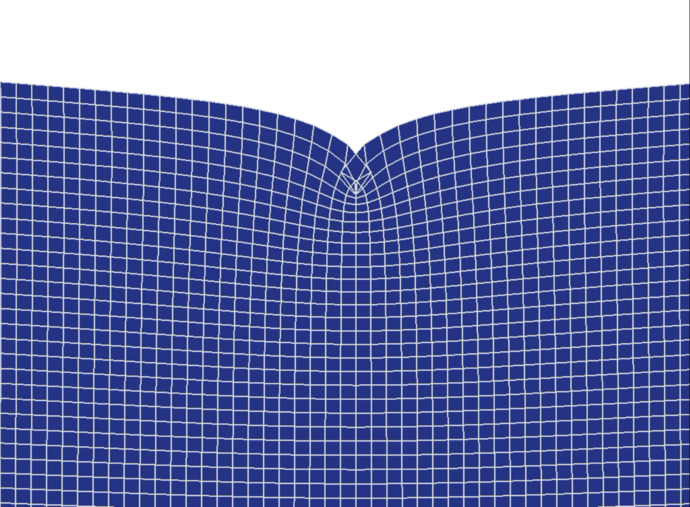
\includegraphics[width=4.5cm]{images/freesurface/b10}}\\
{\tiny Example of a free surface evolution above a sinking sphere. The isostatic rebound above the sphere 
generates a cusp which, if no special measure is taken, ultimately leads to a bow-tied element. Once this 
occurs the simulation stops since the mapping of the bow-tied element to the reference element yields to
wrong elemental matrix. Curtesy of M. Fraters}
\end{center}

In the mildest cases this does not occur but it has long been established that 
large mesh deformation yields low accuracy calculations, 
especially when angles between edges become small or large. 
One way to overcome this problem is to remesh, i.e. generate a better mesh based on the 
available information on the deformed one. In 2D this is routinely done, especially when 
triangular elements are used. In 3D, multiple remeshing are very costly and it is generally
avoided.  
Note also that re-meshing often involves some form of interpolation and therefore some unwanted 
numerical diffusion. 
When deformation is reasonably small, fully lagrangian methods work and have been used in 
geodynamics \cite{hach96b,mera80,labp00}.

\begin{center}
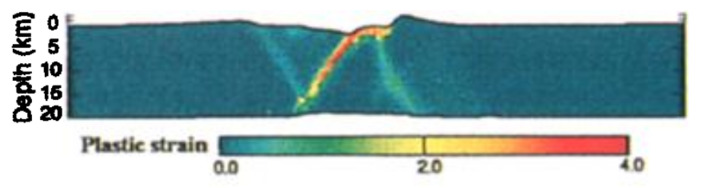
\includegraphics[width=8cm]{images/freesurface/labp00}\\
{\captionfont Taken from \cite{labp00}. Upper-crustal faulting, note that the bottom and the top surface are deformed.}
\end{center}


\begin{center}
\begin{minipage}{0.45\textwidth}
\centering
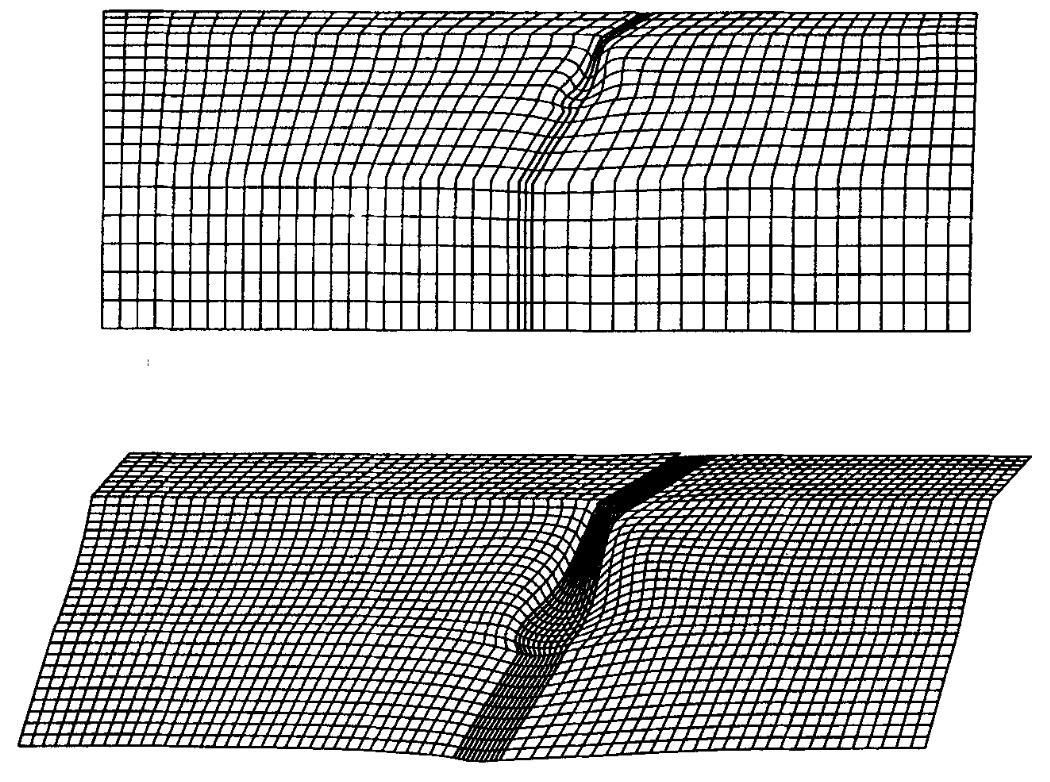
\includegraphics[width=7cm]{images/freesurface/guez96}\\
{\captionfont Taken from \cite{guez96}. Subduction model, topographic expression is shown without vertical exaggeration}. 
\end{minipage}\hfill
\begin{minipage}{0.45\textwidth}
\centering
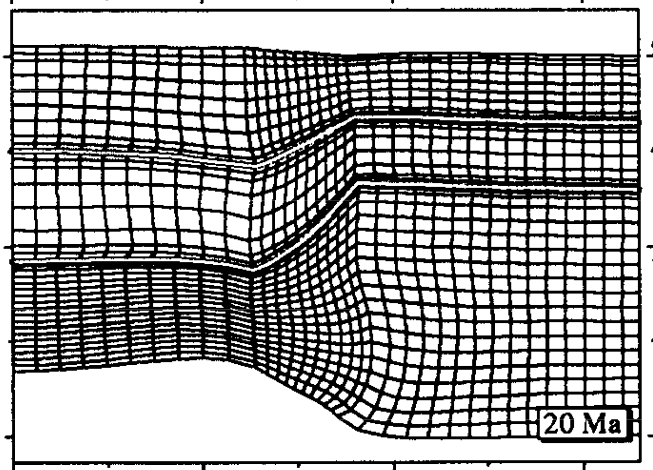
\includegraphics[width=6cm]{images/freesurface/gowo93}\\
{\captionfont Taken from \cite{gowo93}. Asymmetric lithospheric extension.}
\end{minipage}
\end{center}







GET:
Crook et al. 2006, and references therein \cite{crwy06})
Beaumont et al. 1994;  \cite{befh94}


%.......................................
\subsubsection{The Eulerian approach: using sticky air}
\index{general}{Sticky Air}

Sticky air is the default option for numerical methods which mesh 
cannot be deformed (typically the finite difference method).
In this case, the air above the crust/sediments is modelled as a zero-density fluid with 
very low viscosity (see for instance the early article by Zaleski and Julien \cite{zaju92}). 
One problem quickly arises when one realises that the viscosity of the 
air ($\sim 18.5\cdot10^{-6}$ Pa$\cdot$s\footnote{\url{https://en.wikipedia.org/wiki/Viscosity}})
is almost 25-30 orders of magnitude lower than the (effective) viscosity of Earth materials. 
Real air viscosity cannot therefore be used because of 1) round-off errors, 2) extremely 
poorly-conditioned matrices. Low viscosities around $10^{16}-10^{19}$Pa$\cdot$s are then 
commonly used as they are still negligible next to those of the (plastic) crust, and the 
flow of air parallel to Earth materials only generates extremely small shear and normal stress values
(thereby approaching the true nature of a free surface). 
This approach is the one employed in all the papers based on the I2/I3(EL)VIS code (see Appendix~\ref{app:codes})
and has been benchmarked in Crameri et al. \cite{crsg12}.

This approach has a few advantages:
\begin{enumerate}
\item it is simple to implement 
\item it is compatible with all the standard numerical methods (FEM, FDM,FVM)
\item it avoids (potentially complicated) remeshing
\end{enumerate}
and quite a few drawbacks:
\begin{enumerate}
\item it increases the size of the computational domain, thereby adding more unknowns to the linear system: in \cite{scbe08} the air layer is set to 50km while the lithospheric domain underneath is 700km thick;
\item it requires the use of averaging all along the free-surface
where very large viscosity contrasts are present. Here is what Poliakov and Podlachikov \cite{popo92}
say about the sticky air method:
"Zaleski \& Julien \cite{zaju92} used a top layer with a very low
viscosity and density to represent air or water above the
surface. This allows a simple representation of the free
surface. However, due to the very high viscosity and density
contrast and diffusion between the top layer and the
underlying layers, calculations sometimes become unstable
and give significant errors."

\item it can showcase air entrainment:
\begin{center}
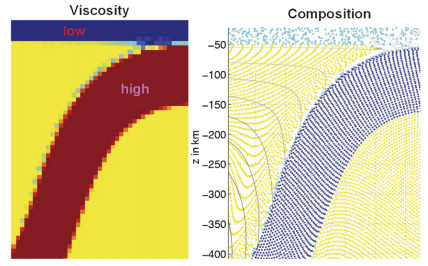
\includegraphics[width=8cm]{images/freesurface/scbe08}\\
{\small Taken from \cite{scbe08}. Details of the entrainment and lubrication of the soft surface layer. 
Light blue particles are sticky air particle and are found to greatly alter the viscosity
of the subduction channel.}
\end{center}
\item it is not clear how thick the air layer must be
\item it often requires to ascribe thermal parameters to the air;
\item it makes the implementation of Dirichlet or Neuman boundary conditions for temperature at the surface less
obvious.
\item it makes the coupling with surface processes codes less straightforward.
\item its accuracy depends on the method used to track materials in the rest of the code (markers, level sets, ...). If markers are used, the free surface position is then known up to the average distance between markers.
\item it negatively impacts the condition number of the matrix.
\end{enumerate}

The sticky air approach is employed by various codes in the subduction benchmark study \cite{scbe08}

The term 'sticky water' is sometimes employed too. The dynamic viscosity of water is about 
$10^{-3}$Pa$\cdot$s so that it is also negligible compared to the viscosity of Earth materials
and the same reasonng as air applies. However, in such a case a density of about 1000kg/m$^3$ 
is then assigned to the layer. REF?

In conclusion, as stated in \cite{crsg12}: "the sticky air method is a good way to
simulate a free surface for Eulerian approaches, provided that its
parameters are chosen carefully."


%..........................................................
\subsubsection{The Arbitrary Lagrangian Eulerian (ALE) approach}
\index{general}{Arbitrary Lagrangian Eulerian} \index{general}{ALE}

It is a very widely used approach in FEM-based geodynamics codes but originates in the field of 
CFD \cite{hiac74,hulz81} and is described at length in \cite{sozo01,dohp04,dohu03}.
To put it very simply, the key idea in the ALE formulation is
the introduction of a computational mesh which can move and deform with a velocity 
independent of the velocity carried by the material particles.

\paragraph{The simple approach in \cite{thie11}.}
What follows is written with a 2D Cartesian model in mind ($Q_1\times P_0$ elements are used).
The computational domain is a rectangle of size $L_x \times  L_y$ 
and a nnx $\times$ nny rectangular grid spanning the simulation
domain is generated.
The grid points constituting the top row of the grid define the
discrete free surface of the domain. Once the Eulerian velocity field
has been computed on these, their position is first updated using a
simple Eulerian advection step (see a,b on figure hereunder):
\[
\vec{r}_i'(t+\delta t) = \vec{r}_i(t) + \vec{v}_i \cdot \delta t
\qquad\qquad
i=1,\dots nnx
\]
The other boundaries of the system remain fixed at locations
$x=0$, $x=L_x$ and $y=0$. Even though the Eulerian grid must conform
to the current domain shape, only vertical motion of grid nodes is
allowed. It is therefore necessary to resample the predicted free
surface given by $\vec{r}_i'$ at equidistant positions between $x=0$ and $x=L_x$.
The resampling is carried out either with Spline functions or a 
moving least square algorithm. 
Finally, the vertical position of all the nodes corresponding
to column $i\in [1,nnx]$ is recalculated so that they are equidistant, 
as sketched in Figure d. This has the advantage of keeping
the mesh distortion to a minimum in the case of large
deformation.

\begin{center}
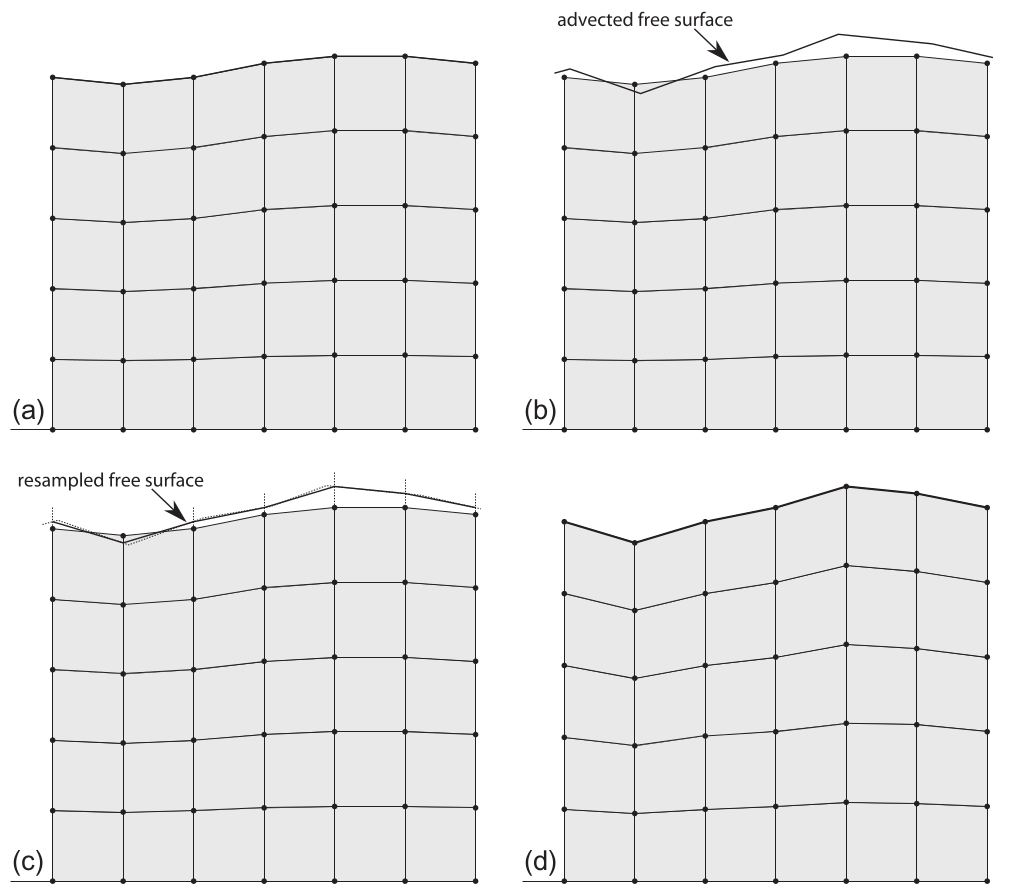
\includegraphics[width=9cm]{images/freesurface/ale2d}\\
 {\small The ALE algorithm of \cite{thie11} in 2D. 
(a) Grid and free surface at a given time $t$; 
(b) advection of the free surface; 
(c) resampling of the free surface at equidistant abscissae; 
(d) vertical adjustment of grid nodes in each column at equidistant ordinates.}
\end{center}

The ALE method is used in the SOPALE, SULEC, FANTOM, ELEFANT, and ASPECT codes to name a few
(see Appendix~\ref{app:codes}).


\paragraph{The not-so-simple but rather elegant approach of ASPECT}

What follows is mostly borrowed from Rose et al \cite{robh17}. Their approach 
has the advantage that it does not presuppose a geometry (Cartesian, Spherical, ...)
nor a number of dimensions. It is also designed to work in parallel and on octree-based
meshes, and with various combinations of boundary conditions.
Note that the authors specify that "for moderate mesh deformation, the mesh stays smooth and well
conditioned, though it breaks down for large deformations".


This approach is obtained by simply imposing the obvious condition 
that no particle (fluid parcel) can cross the free surface (because it is a material surface). 
This can be imposed in a straightforward manner by using a Lagrangian description along this surface. 
However, this condition may be relaxed by imposing only the necessary 
condition: $\vec{\upnu}$ equal to zero along the normal to the boundary 
(ie. $\vec{n}\cdot\vec{\upnu} = 0$, where $\vec{n}$ is the outward unit 
normal to the fluid domain). 
The mesh position, normal to the free surface, is determined from the normal component of 
the particle velocity 
and remeshing can be performed along the tangent; 
see, for instance Huerta and Liu, 1989 \cite{huli88} or Braess and Wriggers, 2000 \cite{brwr00} 

As mentioned above the mesh velocity in normal direction at the free surface (with
unit normal $\vec{n}$) has to be consistent with the velocity of the Stokes
velocity solution $\vec{\upnu}(t)$:
\begin{equation}
\vec{\upnu}_{\text{mesh}}(t)\cdot \vec{n} = \vec{\upnu}(t)\cdot \vec{n} 
\qquad
\text{on}
\quad
\Gamma_F
\end{equation}
In ALE calculations the internal mesh velocity is usually undetermined, 
but one wants to smoothly deform the mesh so as to preserve its regularity, 
avoiding inverted or otherwise poorly conditioned cells. 
The mesh deformation can be calculated in many different ways, icluding algebraic 
(as mentioned in the previous paragraph) and PDE based approaches.
The latter is chosen here. 
The Laplace equation is solved where the unknown is the mesh velocity, i.e. 
one must solve:
\begin{equation}
\Delta \vec{\upnu}_{\text{mesh}} = 0\label{eq:fsaspect1}
\end{equation}
subjected to the following boundary conditions:
\begin{eqnarray}
\vec{\upnu}_{\text{mesh}} &=& \vec{0} \qquad\qquad \text{on } \Gamma_0 \\
\vec{\upnu}_{\text{mesh}} &=& (\vec{\upnu}\cdot\vec{n})\vec{n} \qquad \text{on } \Gamma_F \\
\vec{\upnu}_{\text{mesh}}\cdot \vec{n} &=& 0 \qquad\qquad \text{on } \Gamma_{FS} \label{eq:fsaspect2}
\end{eqnarray}
where $\Gamma_{FS}$ is the part of the boundary with free slip boundary conditions, 
$\Gamma_0$ is the no-slip part and $\Gamma_{FS}$ is the free slip part.

Once the mesh velocity has been obtained for all mesh points, these can be moved with 
said velocity. However, it must be noted that the multiple occurences of the normal vector
in the above equations is not without problem as the normal vectors are not well defined on the
mesh vertices, which is where the mesh velocity is defined.

This yields what the author coin the 'quasi-implicit' scheme 
(we have so far neglected any kind of stabilisation):
\begin{enumerate}
\item Solve the Stokes system;
\item Solve for the surface mesh velocity using Equation~\ref{eq:fsaspect3};
\item Solve for the internal mesh velocity using Equations~\ref{eq:fsaspect1}, \ref{eq:fsaspect2}; 
\item Advect the mesh forward in time using displacements determined by
the forward Euler scheme: $\vec{x}(t^{n+1} ) = \vec{x}(t^n ) + \vec{\upnu}_{\text{mesh}} \delta t$.
\end{enumerate}

Note that Rose et al (2017) \cite{robh17} go further than this, propose a 'nonstandard finite difference scheme' 
and make a link with the stabilisation presented in Kaus et al (2010) \cite{kamm10}.

The authors list two simple methods of computing the normals:
\begin{itemize}
\item one can take $\vec{n}$ as the direction of the local vertical,
\item one could compute $\vec{n}$ as some weighted average of the cell normals adjacent to a given
vertex
\end{itemize}
but conclude that they have found that these schemes do not necessarily
have good mass conservation properties.

A better approach is proposed in the form of an $L_2$ projection of the 
normal velocity $\vec{v}\cdot\vec{n}$ onto the free surface $\Gamma_F$. 
Multiplying the boundary conditions 
\[
\vec{\upnu}_{\text{mesh}} = (\vec{\upnu}\cdot\vec{n})\vec{n} 
\]
by a test function $\vec{w}$ and integrating over the free surface part of the boundary, we find:
\begin{equation}
\int_{\Gamma_F} \vec{w}\cdot\vec{\upnu}_{\text{mesh}} d\Gamma 
=
\int_{\Gamma_F} \vec{w}\cdot (\vec{\upnu}\cdot\vec{n})\vec{n} d\Gamma
=
\int_{\Gamma_F} (\vec{w}\cdot\vec{n}) (\vec{\upnu}\cdot\vec{n}) d\Gamma \label{eq:fsaspect3}
\end{equation}
When discretized, this forms a linear system which can be solved for the mesh velocity 
$\vec{\upnu}_{\text{mesh}}$ at the free surface. 
This system, being nonzero over only the free surface, is relatively computationally inexpensive to solve.
The authors unfortunately fail to mention that this approach is particularly 
interesting since the numerical quadrature used to compute the above integrals
require the normal $\vec{n}$ between the nodes and these normals are well defined over each 
segment joining two nodes!\footnote{what if $Q_k$ with $k>1$ elements are used and nodes on the surface
no more form a line? }

In what follows I present in some detail how to carry out the $L_2$ projection to arrive at the surface velocity
for both $Q_1$ and $Q_2$ elements.

I start from the following integral over a $Q_1$ element:
\begin{eqnarray}
\int_{\Gamma_e} N_i \vec{\upnu}_{mesh} d\Gamma
&=& \int N_i \left( \begin{array}{c} u_{mesh} \\ v_{mesh} \end{array} \right) d\Gamma \\
&=& \int N_i 
\left( \begin{array}{cccc}  N_1 & 0 & N_2 & 0 \\ 0 & N_1 & 0 & N_2  \end{array}\right)\cdot
\left( \begin{array}{c} u_1 \\ v_1 \\ u_2 \\ v_2 \end{array} \right) d\Gamma \\
\end{eqnarray}
Writing this equation alternatively for $N_i=N_1,N_2$ yields:
\[
\int_{\Gamma_e} 
\left( \begin{array}{cccc}  
N_1N_1 & 0 & N_1N_2 & 0 \\ 
0 & N_1N_1 & 0 & N_1N_2 \\
N_2N_1 & 0 & N_2N_2 & 0 \\ 
0 & N_2N_1 & 0 & N_2N_2 
\end{array}\right)
\cdot \left( \begin{array}{c} u_1 \\ v_1 \\ u_2 \\ v_2 \end{array} \right) 
d\Gamma 
=
\int_{\Gamma_e} 
\left( \begin{array}{cccc}  
N_1N_1 & 0 & N_1N_2 & 0 \\ 
0 & N_1N_1 & 0 & N_1N_2 \\
N_2N_1 & 0 & N_2N_2 & 0 \\ 
0 & N_2N_1 & 0 & N_2N_2 
\end{array}\right)
d\Gamma \quad 
\cdot \left( \begin{array}{c} u_1 \\ v_1 \\ u_2 \\ v_2 \end{array} \right) 
\]
Turning now to the right hand side %(I denote by $\vec{n}_e$ the normal to the element edge):
$\int_{\Gamma_e} N_i   (\vec{\upnu}\cdot\vec{n}_e)\vec{n}_e  d\Gamma$, it yields the following rhs:
\[
\int_{\Gamma_e}   (\vec{\upnu}\cdot\vec{n}_e)
\left(\begin{array}{c}
N_1 n_x \\ N_1 n_y \\ N_2 n_x \\ N_2 n_y
\end{array}\right)
 d\Gamma
\]
The elemental matrix and rhs must be built for each element and assembled in a 
global matrix and rhs. The solution is the mesh velocity vector at all surface nodes.
the same approach can be taken for $Q_2$ elements:
\begin{eqnarray}
\int_{\Gamma_e} N_i \vec{\upnu}_{mesh} d\Gamma
&=& \int N_i \left( \begin{array}{c} u_{mesh} \\ v_{mesh} \end{array} \right) d\Gamma \\
&=& \int N_i 
\left( \begin{array}{cccccc}  
N_1 & 0 & N_2 & 0 & N_3 & 0\\ 
0 & N_1 & 0 & N_2 & 0 & N_3 
\end{array}\right)\cdot
\left( \begin{array}{c} u_1 \\ v_1 \\ u_2 \\ v_2 \\ u_3 \\ v_3 \end{array} \right) d\Gamma 
\end{eqnarray}
Writing this equation alternatively for $N_i=N_1,N_2,N_3$ yields:
\begin{eqnarray}
&&\int_{\Gamma_e} 
\left( \begin{array}{cccccc}  
N_1N_1 & 0 & N_1N_2 & 0 & N_1N_3 & 0 \\ 
0 & N_1N_1 & 0 & N_1N_2 & 0 & N_1N_3 \\
N_2N_1 & 0 & N_2N_2 & 0 & N_2N_3 & 0 \\ 
0 & N_2N_1 & 0 & N_2N_2 & 0 & N_2N_3 \\
N_3N_1 & 0 & N_3N_2 & 0 & N_3N_3 & 0 \\ 
0 & N_3N_1 & 0 & N_3N_2 & 0 & N_3N_3 \\
\end{array}\right)
\cdot \left( \begin{array}{c} u_1 \\ v_1 \\ u_2 \\ v_2 \\ u_3 \\ v_3 \end{array} \right) 
d\Gamma \nn\\ 
&=&
\int_{\Gamma_e} 
\left( \begin{array}{cccccc}  
N_1N_1 & 0 & N_1N_2 & 0 & N_1N_3 & 0 \\ 
0 & N_1N_1 & 0 & N_1N_2 & 0 & N_1N_3 \\
N_2N_1 & 0 & N_2N_2 & 0 & N_2N_3 & 0 \\ 
0 & N_2N_1 & 0 & N_2N_2 & 0 & N_2N_3 \\
N_3N_1 & 0 & N_3N_2 & 0 & N_3N_3 & 0 \\ 
0 & N_3N_1 & 0 & N_3N_2 & 0 & N_3N_3 
\end{array}\right)
d\Gamma \quad 
\cdot \left( \begin{array}{c} u_1 \\ v_1 \\ u_2 \\ v_2 \\ u_3 \\ v_3 \end{array} \right) 
\end{eqnarray}

The right hand side is then  
\[
\int_{\Gamma_e}   (\vec{\upnu}\cdot\vec{n}_e)
\left(\begin{array}{c}
N_1 n_x \\ N_1 n_y \\ 
N_2 n_x \\ N_2 n_y \\
N_3 n_x \\ N_3 n_y 
\end{array}\right)
 d\Gamma
\]
Having obtained the boundary condition velocity for the Laplace equation, we can now turn our attention 
to solving this ODE. 


Note that Rose et al (2017) \cite{robh17} go further than this and propose a 'nonstandard finite difference scheme' and make a link with the stabilisation presented in Kaus et al (2010) \cite{kamm10}.

In what follows I omit the subscript 'mesh' and focus on the 2D case. The components of the (mesh) velocity
are given by
\[
u^h = \sum_{i=1}^{m_\upnu} N_i^\upnu u_i
\qquad
\qquad
v^h = \sum_{i=1}^{m_\upnu} N_i^\upnu v_i
\qquad
\qquad
\vec{\upnu}^h=\left( 
\begin{array}{c}
u^h \\
v^h 
\end{array}  \right)
\]
We start from the ODE to solve in its strong form:
\[
\Delta \vec{\upnu}^h = \vec{0}
\]
We multiply it by a velocity test function $N_i^\upnu$ and integrate over an element: 
\begin{eqnarray}
&&\vec 0 \nonumber\\
&=& \int_{\Omega_e} N_i^\upnu  \Delta \vec{\upnu}^h \nonumber\\ 
&=&\int_{\Omega_e} N_i^\upnu \Delta \vec\upnu^h dV \nonumber\\
&=&\int_{\Omega_e}  \left(\begin{array}{c}
N_i^\upnu \Delta u^h \\
N_i^\upnu \Delta v^h 
\end{array}\right) dV \nonumber\\
&=&\int_{\Omega_e}  \left(\begin{array}{c}
N_i^\upnu \vec\nabla \cdot \vec\nabla u^h \\
N_i^\upnu \vec\nabla \cdot \vec\nabla v^h 
\end{array}\right) dV \nonumber\\
&=&
\int_{\Omega_e}   \left(\begin{array}{c}
\vec\nabla N_i^\upnu \cdot \vec\nabla u^h \\
\vec\nabla N_i^\upnu \cdot \vec\nabla v^h 
\end{array}\right) dV \nonumber\\
&=&
\int_{\Omega_e}
\left(\begin{array}{c}
\partial_x N_i^\upnu \partial_x u^h + \partial_y N_i^\upnu \partial_y u^h \\ 
\partial_x N_i^\upnu \partial_x v^h + \partial_y N_i^\upnu \partial_y v^h 
\end{array}\right) dV \nonumber\\
&=&\int_{\Omega_e}
\left(
\begin{array}{cccc}
\partial_x N_i^\upnu & \partial_y N_i^\upnu & 0 & 0 \\ 
0 & 0 & \partial_x N_i^\upnu & \partial_y N_i^\upnu  \\ 
\end{array}
\right)
\!\cdot\!
\left(
\begin{array}{c}
\partial_x u^h \\
\partial_y u^h \\
\partial_x v^h \\
\partial_y v^h 
\end{array}
\right) dV \nonumber\\
&=&\int_{\Omega_e}
\left(
\begin{array}{cccc}
\frac{\partial N_i^\upnu}{\partial x} & \frac{\partial N_i^\upnu}{\partial y} & 0 & 0 \\ 
0 & 0 & \frac{\partial N_i^\upnu}{\partial x} & \frac{\partial N_i^\upnu}{\partial y}  \\ 
\end{array}
\right)
\!\cdot\!
\left(
\begin{array}{cccccccccc}
\frac{\partial N_1^\upnu}{\partial x} & 0  & \frac{\partial N_2^\upnu}{\partial x} & 0  & \cdots & \frac{\partial N^\upnu_{m_\upnu}}{\partial x} & 0 \\ \\
\frac{\partial N_1^\upnu}{\partial y} & 0  & \frac{\partial N_2^\upnu}{\partial y} & 0  & \cdots & \frac{\partial N^\upnu_{m_\upnu}}{\partial y} & 0 \\ \\
0 & \frac{\partial N_1^\upnu}{\partial x}  & 0& \frac{\partial N_2^\upnu}{\partial x}  & \cdots & 0 & \frac{\partial N^\upnu_{m_\upnu}}{\partial x}  \\ \\
0 & \frac{\partial N_1^\upnu}{\partial y}  & 0& \frac{\partial N_2^\upnu}{\partial y}  & \cdots & 0 & \frac{\partial N^\upnu_{m_\upnu}}{\partial y}  
\end{array}
\right) 
\!\cdot\!
\left(
\begin{array}{c}
u_1 \\ v_1 \\ u_2 \\ v_2 \\ \dots \\ u_{m_v} \\ v_{m_v} 
\end{array}
\right) dV \nonumber
\end{eqnarray}
Writing this equation for $i=1,...m_\upnu$, we obtain:
\[
\int
\left(
\begin{array}{cccc}
\frac{\partial N_1^\upnu}{\partial x} & \frac{\partial N_1^\upnu}{\partial y} & 0 & 0 \\ 
0 & 0 & \frac{\partial N_1^\upnu}{\partial x} & \frac{\partial N_1^\upnu}{\partial y}  \\ 
\frac{\partial N_2^\upnu}{\partial x} & \frac{\partial N_2^\upnu}{\partial y} & 0 & 0 \\ 
0 & 0 & \frac{\partial N_2^\upnu}{\partial x} & \frac{\partial N_2^\upnu}{\partial y}  \\ 
\vdots & \vdots & \vdots & \vdots \\
\vdots & \vdots & \vdots & \vdots \\
\frac{\partial N_{m_\upnu}^\upnu}{\partial x} & \frac{\partial N_{m_\upnu}^\upnu}{\partial y } & 0 & 0 \\ 
0 & 0 & \frac{\partial N_{m_\upnu}^\upnu}{\partial x} & \frac{\partial N_{m_\upnu}^\upnu}{\partial y}  \\ 
\end{array}
\right)
\cdot
\left(
\begin{array}{cccccccccc}
\frac{\partial N_1^\upnu}{\partial x} & 0  & \frac{\partial N_2^\upnu}{\partial x} & 0  & \cdots & \frac{\partial N^\upnu_{m_\upnu}}{\partial x} & 0 \\ \\
\frac{\partial N_1^\upnu}{\partial y} & 0  & \frac{\partial N_2^\upnu}{\partial y} & 0  & \cdots & \frac{\partial N^\upnu_{m_\upnu}}{\partial y} & 0 \\ \\
0 & \frac{\partial N_1^\upnu}{\partial x}  & 0& \frac{\partial N_2^\upnu}{\partial x}  & \cdots & 0 & \frac{\partial N^\upnu_{m_\upnu}}{\partial x}  \\ \\
0 & \frac{\partial N_1^\upnu}{\partial y}  & 0& \frac{\partial N_2^\upnu}{\partial y}  & \cdots & 0 & \frac{\partial N^\upnu_{m_\upnu}}{\partial y}  
\end{array}
\right) 
\cdot
\underbrace{
\left(
\begin{array}{c}
u_1 \\ v_1 \\ u_2 \\ v_2 \\ \dots \\ u_{m_v} \\ v_{m_v} 
\end{array}
\right) }_{\vec V}
dV
=\vec{0}
\]
or, 
\[
\left( \int_{\Omega_e} {\bm B}^T  \cdot {\bm B} \; dV \right)\cdot \vec{V} = \vec{0}
\]
where ${\bm B}$ is a $(ndim*ndim) \times (m_v*ndofV)$ matrix. This is implemented in Stone 54 \ref{f54}.

\begin{remark}
The integration by parts should have a minus appear but since the left hand side 
is 0, it is not taken into account. 
\end{remark}

\todo[inline]{surface terms arising from the integration by parts are neglected. EXPLAIN WHY!}


\paragraph{Yet another approach \cite{dohp04}}
The unknown position of free surfaces can be computed using the following approach:
for the simple case of a single-valued function $h=h(x,y,t)$, a hyperbolic equation must be solved,
\begin{equation}
\frac{\partial h}{\partial t} + (\vec{ \upnu}\cdot \vec{ \nabla}) h = 0    \label{eqfs1}
\end{equation}
This is the kinematic equation of the surface and has been used, for instance, 
by Ramaswamy and Kawahara (1987), Huerta and Liu, 1988b, 1990; Souli and Zolesio (2001).





\underline{Idea:} Eq. (\ref{eqfs1}) is a simple advection equation. 
One could also add a diffusion operator with a diffusion coefficient $D$.
Low values of $D$ could be used to stabilise the surface while 
higher values (possibly nonlinear ones) could be used to account for simple 
surface processes. 

\begin{equation}
\frac{\partial h}{\partial t} + (\vec{\upnu}\cdot\vec{ \nabla}) h = D \Delta h  \label{eqfs2}
\end{equation}

Also, Hansen and Nielsen \cite{hanl00,hani03} write:
During the entire model evolution surface processes act to re-distribute sediments. 
These processes are modelled by a diffusion equation with a source term enabling the transport 
of sediments to and from the model profile. The transport equation is written
\[
\dot{h}=\nabla\cdot (\kappa \nabla h) + \dot{s}(w)
\]
where $\kappa=200 km^2/Ma$ is the diffusivity of topography and $\dot{s}(w)$ 
is a linear function of water depth. 



The following pictures are taken from Naliboff et al \cite{nabp17} on the topic 
of how complex fault interaction controls continental rifting. It is a beautiful
example (among many) of the importance of free surface geodynamical expression
and large deformation:

\begin{center}
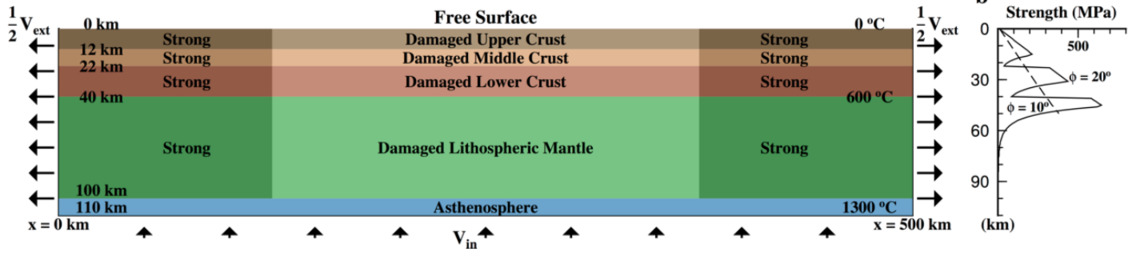
\includegraphics[width=9cm]{images/freesurface/nabp17a}\\
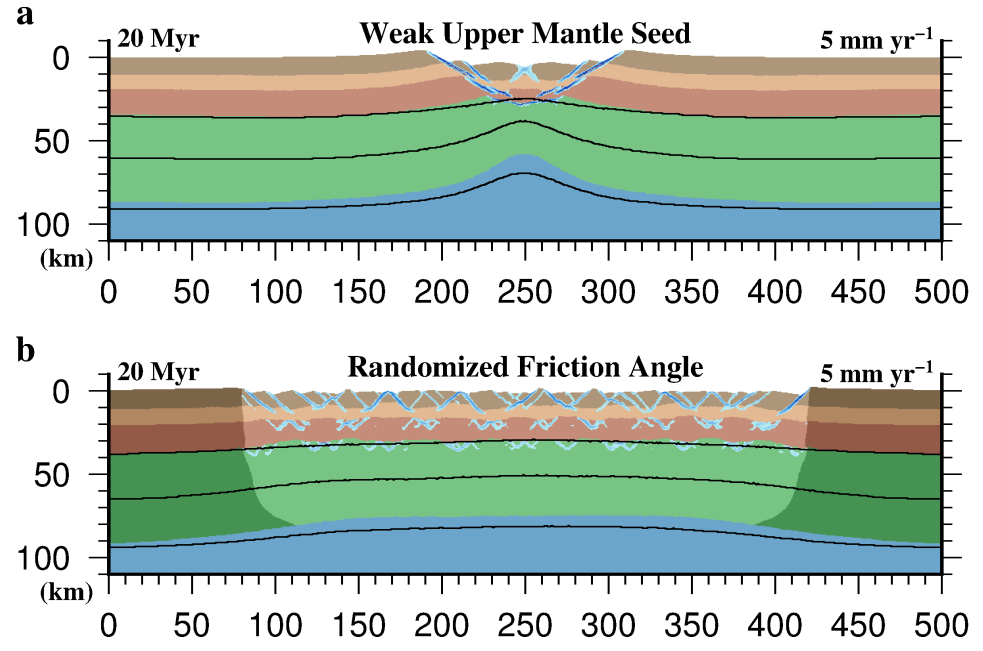
\includegraphics[width=9cm]{images/freesurface/nabp17b}\\
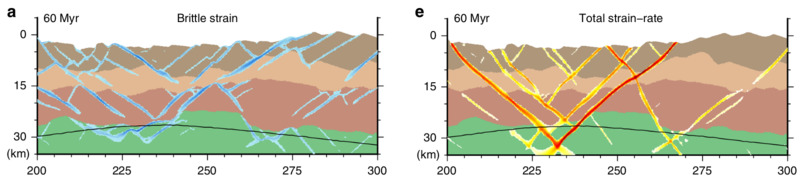
\includegraphics[width=14cm]{images/freesurface/nabp17c}\\
{\captionfont Taken from \cite{nabp17}}
\end{center}

%-------------------------------------------------------
\subsubsection{On the topic of moving internal nodes}

Braess \& Wriggers \cite{brwr00} propose the following interesting algorithm:
"A measure of the quality of a triangular mesh is the quotient of the
outer radius $r_{out}$ and the inner radius $r_{in}$ 
of each element. This quotient is important because it plays a
certain role in a priori error estimates. If an element degenerates this quotient will approach infinity.
Another important feature of good mesh is that no element becomes very large. With these considerations
in mind the penalty function $W$ is defined:
\begin{equation}
W = \sum_{elts} \left( \frac{r_{out}}{r_{in}} \right)^m \left( \frac{r_{out}}{r_0} \right)^n
\end{equation}
where $m$, $n$ and $r_0$ are positive constants. 
For our calculations we chose $m=3$, $n=1$ and $r_0=1$, but the results seem
to depend only slightly on this choice. Whenever a triangle is distorted or very large, this function becomes
very large. A similar penalty function was presented in \cite{jole97} for 
four-node elements. In that case the angles
of the elements are used to construct the penalty function.
In order to regularize a distorted mesh the coordinates of the internal nodes will be chosen such that $W$ is
minimized. It is not necessary to reach the global minimum, a rough approximation is sufficient.
Therefore the minimization of the potential can be done efficiently with standard procedures and will not be
discussed in any detail. This algorithm can also be applied to $h$-adaptive mesh-generation by choosing
appropriate constants $r_0$ for each triangle."\footnote{Indeed, if $r_0$ is the same for all elements
this parameter will not play any role at all in the minimisation process.} 



\vspace{4cm}
This is still WORK IN PROGRESS. I Need to look at those papers:
\cite{raka87}
\cite{huli88}\cite{pobe98}
\cite{bens89}
\cite{sucy00}
\cite{rama90}
\cite{tebm92}(moving pulse)
\cite{dumg11}
\cite{dumy16} 
\cite{anmp15}
\cite{krwd12}
\cite{stcl10}
\cite{maie12}
\cite{guez96}\cite{zhgm96}
\cite{elsp04}
\cite{brwr00}
\cite{pada83}
and talk about free surface stabilisation \cite{kamm10,qube11,dumg11,robh17}.



